\subsection{Implementation of \astarix and \dijkstra}
Our \astarix implementation uses an adjacency list graph data structure to
represent the reference and the trie in a unified way, representing each letter
by a separate edge object.
%\para{Reverse Complement Alignment}
To represent the reverse complementary walks in $\RG$, the vertices are doubled,
connected in the opposite direction, and labeled with complementary nucleotides
($\texttt{A} \leftrightarrow \texttt{T}$, $\texttt{C} \leftrightarrow
\texttt{G}$).
%
%\para{Default Parameters}
We do not limit the number of memoized heuristic function values
(\cref{TRIEpara:memoization}), but note we could do so by resetting the memoization
table periodically.
%
Our implementation of \dijkstra reuses the same \astarix codebase except the
use of a heuristic function (\ie, with $h \equiv 0$).

%\para{Optimizations}
We apply all described optimizations to \astarix and \dijkstra, except
\cref{TRIEsubsec:speedup-heuristic,TRIEsubsec:partition} which are applicable only to
\astarix.

\subsection{Parameter tuning for \astarix} \label{TRIEsubsec:parameter_estimation}

While the optimality of \astarix is not affected by its parameters, its
performance is. To compare with other aligners, we use values \mbox{$d=5$},
\mbox{$\costcap=5$}, \mbox{$D = \lfloor \log_\Sigma \lvert \RG \rvert \rfloor$}.
Follows an investigation of the influence of different parameters ($\costcap$,
$d$, $D$) on the runtime and memory usage.

\begin{figure}[b]
	\centering
	\begin{minipage}{0.48\linewidth}
		\centering
		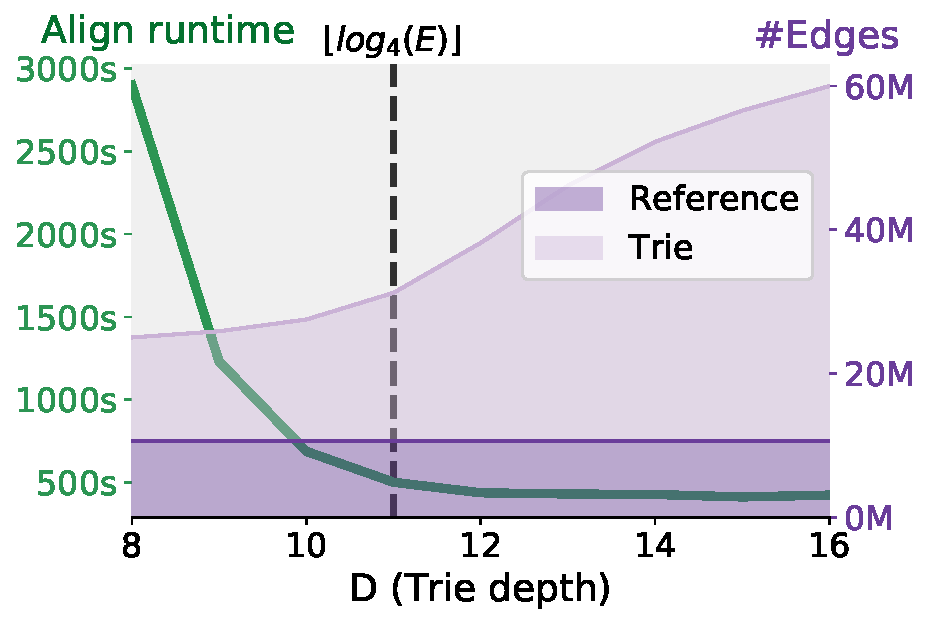
\includegraphics[width=\linewidth]{figs/trie/MHC1-trie-vs-D.pdf}
		\caption{Left: Effect of $D$ on performance of \astarix (MHC1 experiment). The dashed line shows our choice of $D$. Right: Runtime of \astarix depending on $d$ and $\costcap$ (MHC1 experiment).}
		%\label{TRIEsubfig:MHC1-trie_vs_D}
		\label{TRIEfig:trie_vs_D}
	\end{minipage}~\hspace{0.7em}
	\begin{minipage}{0.49\linewidth}
		\centering
		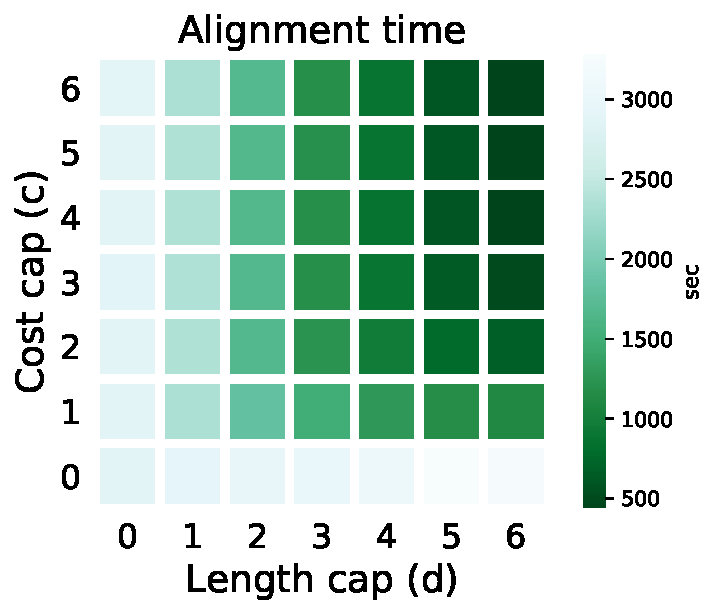
\includegraphics[width=0.8\linewidth]{figs/heuristic/MHC1-heatmap-c_vs_d-align_sec.pdf}
		%\caption{Runtime of \astarix depending on $d$ and $\costcap$ (MHC1 experiment).}
		\label{TRIEfig:heuristic-parameters}
	\end{minipage}
\end{figure}

\cref{TRIEfig:trie_vs_D} demonstrates the benefit of using a trie with the size
reduction optimization (end of \cref{TRIEsubsec:trie}): increasing the trie depth
$D$ speeds up aligning but requires more memory. Selecting the trie depth based
on the graph size \mbox{$D = \lfloor \log_\Sigma \lvert \RG \rvert \rfloor$}
provides a reasonable trade-off between alignment time and memory.

\cref{TRIEfig:heuristic-parameters} shows the joint effect of $\costcap$ and $d$. It
demonstrates that having a long reach ($d$) that covers at least some errors
($\costcap > 0$) is a reasonable strategy for choosing $d$ and $\costcap$.

\subsection{Compared Aligners: \pasgal and \bitparallel}

% Even though there is a variety of short read-to-graph aligners, only a few are
% guaranteed to be optimal.
We compare the performance of \astarix to that of two state-of-the-art optimal
aligners: \pasgal and \bitparallel, with their default parameters.
%
We do not compare to the exact aligner of \vg as (i)~its optimal alignment
is intended for testing purposes only, (ii)~it does not provide an
interface for aligning a set of reads, and (iii)~it has been consistently
outperformed by \pasgal~\cite{jain_accelerating_2019}.

\pasgal is compiled with AVX2 SIMD support. The resulting alignments are not
expected to match exactly between the local aligner \pasgal and the semi-global
aligners (\astarix and \bitparallel) as they solve different tasks with
different edit costs. Nevertheless, in analogy with the evaluations of
\pasgal~\cite{jain_accelerating_2019}, it is still meaningful to compare
performance, assuming that the dynamic programming approach of \pasgal can be
adapted to semi-global alignment with similar performance.

Both \bitparallel and \pasgal reach their worst-case runtime complexity
independent of the edit costs $\Delta=(\cmatch,\csubst,\cins,\cdel)$. \pasgal is
evaluated using its default costs ~$\Delta=(-1,1,1,1)$ and \bitparallel is
evaluated using the only supported costs~$\Delta=(0,1,1,1)$.
